\documentclass{llncs}
\usepackage{amsmath, amssymb, fancyvrb, multirow, color, stmaryrd}
\usepackage{svg}
\usepackage{wrapfig}
\usepackage{graphicx}
\usepackage{fancyvrb}
\usepackage{hyperref}
\usepackage[]{algorithm2e}

\newcommand{\enforce}{\mathsf{enforce}}
\newcommand{\traj}{\mathsf{traj}}
\newcommand{\drh}{\textsf{drh}}
\newcommand{\dReal}{\textsf{dReal}}
\newcommand{\dReach}{\textsf{dReach}}

%\usepackage{multirow}
\usepackage{amsmath,hyperref}
\hypersetup{
    colorlinks,%
    citecolor=blue,%
    filecolor=blue,%
    linkcolor=blue,%
    urlcolor=blue
}
\usepackage{amssymb,verbatim}
\usepackage{fix2col,listings,fancyvrb}
\usepackage{multicol}
\usepackage{graphicx,epsfig}
\usepackage{caption}
\usepackage{stmaryrd}
\usepackage{setspace}
\usepackage{ulem}
\usepackage{newlfont}
\usepackage{epsfig,graphics}
\usepackage{fancybox}
\usepackage{listings}
\usepackage{caption}
\usepackage{graphicx,epsfig}
\usepackage{caption}
\usepackage{makeidx}
\usepackage{listings}
\lstset{
  basicstyle=\ttfamily,
  breaklines=true,
  columns=fullflexible,
  escapeinside = ||,
  breakindent=0pt}
\makeindex

\usepackage{algorithm}
\usepackage{algpseudocode}
\usepackage{hyperref}
\hypersetup{
    colorlinks,%
    citecolor=blue,%
    filecolor=blue,%
    linkcolor=blue,%
    urlcolor=blue
}


%\usepackage[ruled,lined,boxed,commentsnumbered,linesnumbered]{algorithm2e}

\setcounter{secnumdepth}{3}
\setcounter{tocdepth}{2}

\newcommand\bookepigraph[4]{
\vspace{1em}\hfill{}\begin{minipage}{#1}{\begin{spacing}{0.9}
\small\noindent\textit{#2}\end{spacing}
\vspace{1em}
\hfill{}{#3}\\

\vspace{-1em}\begin{flushright}{#4}\end{flushright}}\vspace{2em}
\end{minipage}}

\newcommand{\dom}{\mbox{dom}}

\newcommand\epigraph[3]{
\vspace{1em}\hfill{}\begin{minipage}{#1}{\begin{spacing}{0.9}
\small\noindent\textit{#2}\end{spacing}
\vspace{1em}
\hfill{}{#3}}\vspace{2em}
\end{minipage}}

\newcommand\anonymousepigraph[2]{
\vspace{1em}\hfill{}\begin{minipage}{#1}{\begin{spacing}{0.9}
\small\noindent\textit{#2}\end{spacing}}
\vspace{1em}
\end{minipage}}

\newcommand{\len}{\mathit{len}}
\newcommand{\poly}{\mathsf{poly}}
\newcommand{\N}{\mathbb{N}}
\newcommand{\R}{\mathbb{R}}
\newcommand{\D}{\mathbb{D}}
\newcommand{\cf}{\mathsf{CF}}
\newcommand{\be}{\mathsf{BE}}
\newcommand{\fe}{\mathbb{F}^{[\underline{e}, \overline{e}]}_{\beta,p}}
\newcommand{\rad}{\mathrm{rad}}


\newcommand{\flow}{\mathsf{flow}}
\newcommand{\jump}{\mathsf{jump}}
\newcommand{\inv}{\mathsf{inv}}
\newcommand{\init}{\mathsf{init}}
\newcommand{\guard}{\mathsf{guard}}
\newcommand{\reset}{\mathsf{reset}}
\newcommand{\reach}{\mathsf{Reach}}
\newcommand{\unsafe}{\mathsf{unsafe}}

\newcommand{\safe}{\mathsf{safe}}
\newcommand{\p}{\mathsf{P}}
\newcommand{\np}{\mathsf{NP}}
%\newcommand{\dom}{\mathrm{dom}}


\newcommand\tupleof[1]{\left\langle #1 \right\rangle}
\newcommand\vI{\vec{I}}
\newcommand\va{\vec{a}}
\newcommand\vb{\vec{b}}
\newcommand\vc{\vec{c}}
\newcommand\vd{\vec{d}}
\newcommand\ve{\vec{e}}
\newcommand\vl{\vec{l}}
\newcommand\vu{\vec{u}}
\newcommand\vx{\vec{x}}
\newcommand\vy{\vec{y}}
\newcommand\trp[1]{#1^{{}^{\mbox{\sc{t}}}}}
\newcommand{\lrf}{\mathcal{L}_{\mathbb{R}_{\mathcal{F}}}}
%\usepackage{wrapfigure}

%\doublespacing


\title{\dReach{}: $\delta$-Reachability Analysis for Hybrid Systems}

\begin{document}


\mainmatter  % start of an individual contribution

\author{Soonho Kong, Sicun Gao, Wei Chen, and Edmund Clarke}
\authorrunning{S. Kong, S. Gao, W. Chen,  E. Clarke}
\institute{Computer Science Department, Carnegie Mellon University, USA}
\maketitle

\begin{abstract}
  \dReach{} encodes reachability problems of hybrid systems to
  first-order formulae over real numbers. The formulae are solved by
  delta-decision procedures in the SMT solver \dReal{}. In this way,
  \dReach{} is able to handle a wide range of highly nonlinear hybrid
  systems. Experiments have shown promising results on many nonlinear
  benchmarks that are not solvable by other existing tools.
\end{abstract}

% Tool demonstration papers focus on the usage aspects of tools. As with
% regular tool papers, authors are strongly encouraged to make their
% tools publicly available, preferably on the web. Theoretical
% foundations and experimental evaluation are not required, however, a
% motivation as to why the tool is interesting and significant should be
% provided. Tool demonstration papers can have a maximum of 6 pages.
% They should have an appendix of up to 6 additional pages with details
% on the actual demonstration.

\section{Introduction}\label{sec:intro}

% Need a paragrapgh or two to explain why the tool is interesting and
% significant should be provided.

\dReach{} is a bounded reachability analysis tool for hybrid systems.
It encodes bounded reachability problems of hybrid systems as
first-order formulas over the real numbers, and solves them using
$\delta$-decision procedures in the SMT solver
\dReal{}~\cite{DBLP:conf/cade/GaoKC13}. \dReach{} is able to handle a
wide range of highly nonlinear hybrid systems~\cite{CMSB14,DBLP:conf/fmcad/GaoKC13,DBLP:conf/hybrid/KapinskiDSA14,6868816}.
Figure~\ref{fig:prostate-example} highlights some of its features: on
the left is an example of some nonlinear dynamics that \dReach{} can
handle, and on the right a visualized counterexample generated by
\dReach{} on this model.
\begin{figure}[!h]
  \subfloat[An example of nonlinear hybrid system model: off-treatment
  mode of the prostate cancer treatment model~\cite{CMSB14}\label{subfig-1:prostate}]{
    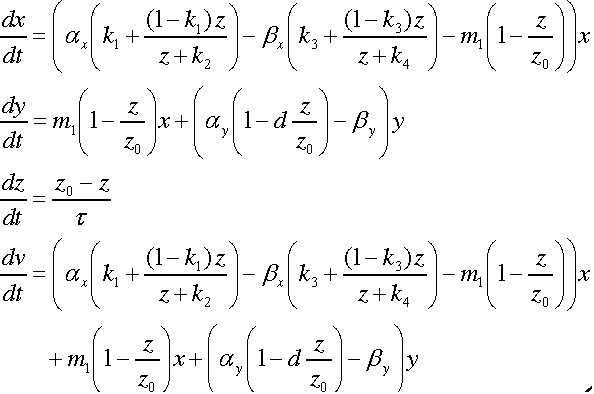
\includegraphics[width=0.45\textwidth]{images/prostatebw-mode2.pdf}
  }
  \hfill
  \subfloat[Visualization of a generated counterexample. Change in the shade of colors represents discrete mode changes.]{%
    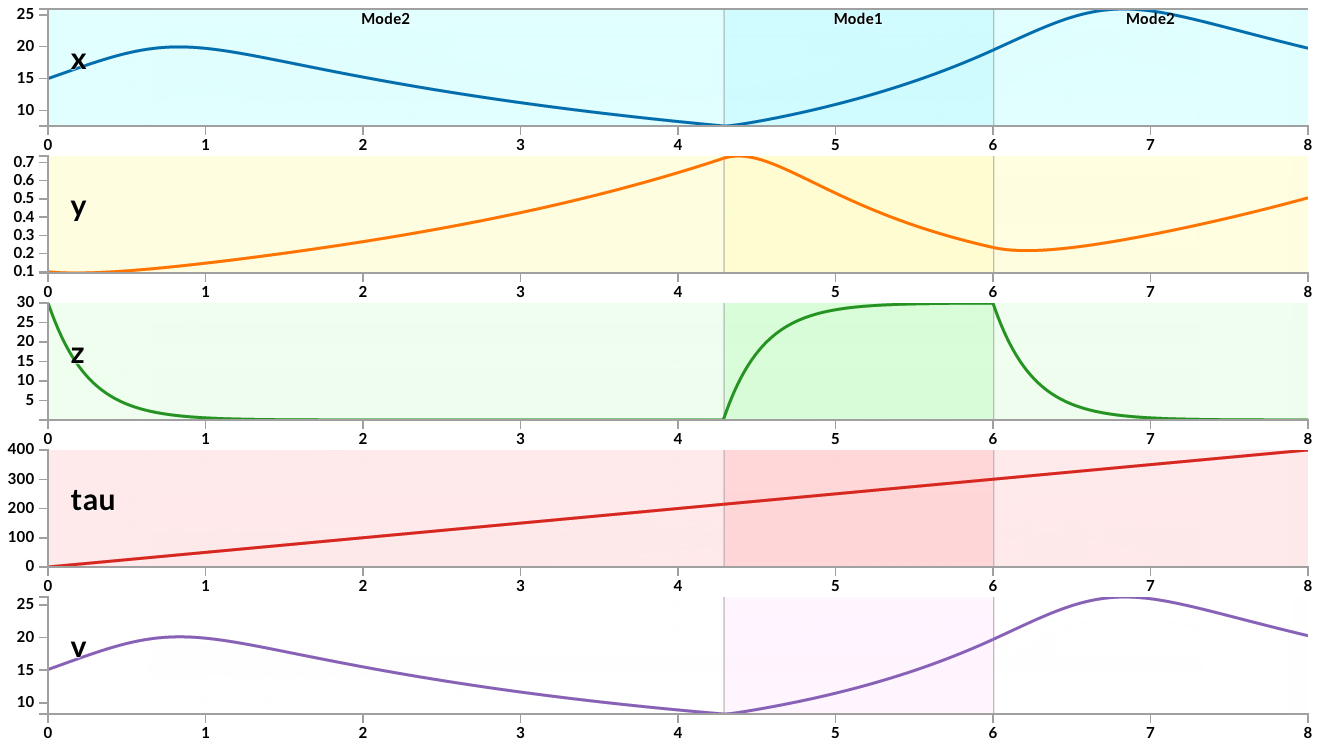
\includegraphics[width=0.48\textwidth]{images/prostate}
  }
  \caption{An example of nonlinear dynamics and counterexample-generation.}
  \label{fig:prostate-example}
\end{figure}

It is well-known that the standard bounded reachability problems for
simple hybrid systems are already highly
undecidable~\cite{DBLP:conf/hybrid/AlurCHH92}.
Instead, we work in the framework of $\delta$-reachability of hybrid systems~\cite{DBLP:journals/corr/GaoKCC14}.
Here $\delta$ is an arbitrary positive rational number, provided by the user to
specify the bound on numerical errors that can be tolerated in the analysis.
For a hybrid system $H$ and an unsafe region $\unsafe$ (both encoded as logic formulas),
the $\delta$-reachability problem asks for one of the following answers:
\begin{itemize}
        \item {\sf safe}: $H$ cannot reach $\unsafe$.
        \item {\sf $\delta$-unsafe}: $H^{\delta}$ can reach $\unsafe^{\delta}$.
\end{itemize}
Here, $H^{\delta}$ and $\unsafe^{\delta}$ encode ($\delta$-bounded) overapproximations
of $H$ and $\unsafe$, defined explicitly as their syntactic variants.%(See Section~\ref{sec:delta-reachability} in the Appendix.)
It is important to note that the definition makes the answers no weaker than standard reachability:
When {\sf safe} is the answer, we know for certain that $H$ does not reach
the unsafe region (no $\delta$ is involved); when {\sf $\delta$-unsafe} is the answer,
we know that there exists some $\delta$-bounded perturbation of the system that can render it unsafe.
Since $\delta$ can be chosen to be very small, {\sf$\delta$-unsafe} answers in fact
discover robustness problem in the system, which should be regarded as unsafe indeed.
We have proved that bounded $\delta$-reachabilty is decidable for a wide range
of nonlinear hybrid systems, even with reasonable complexity bounds~\cite{DBLP:journals/corr/GaoKCC14}.
This framework provides the formal correctness guarantees of \dReach{}.

Apart from solving $\delta$-reachability, the following key features of \dReach{}
distinguish it from other existing tools in this
domain~\cite{DBLP:journals/jlp/FranzleTE10,DBLP:conf/cav/FrehseGDCRLRGDM11,DBLP:journals/tac/AlthoffK14,DBLP:conf/hybrid/Frehse05,DBLP:conf/icons/HerdeEFT08,DBLP:conf/rtss/ChenAS12,DBLP:conf/aaai/CimattiMT12}.
%insert explanations for each item.
\begin{enumerate}
\item Expressiveness. \dReach{} allows the user to describe hybrid
  systems using first-order logic formulas over real numbers with a
  wide range of nonlinear functions. This allows the user to specify
  the continuous flows using highly nonlinear differential equations,
  and the jump and reset conditions with complex Boolean combinations
  of nonlinear constraints. \dReach{} also faithfully translates mode
  invariants into $\exists\forall$ logic formulas, which can be
  directly solved under certain restrictions on the invariants.
\item Property-guided search. \dReach{} maintains logical encodings
  (the same approach as~\cite{DBLP:conf/aaai/CimattiMT12}), whose size
  is linear in the size of the inputs, of the reachable states of a
  hybrid system~\cite{DBLP:journals/corr/GaoKCC14}. The tool searches
  for concrete counterexamples to falsify the reachability properties,
  instead of overapproximating the full reachable states. This avoids
  the usual state explosion problem in reachable set computation,
  because the full set of states does not need to be explicitly
  stored. This change is analogous to the difference between SAT-based
  model checking and BDD-based symbolic model checking.
\item Tight integration of symbolic reasoning and numerical solving.
  \dReach{} delegates the reasoning on discrete mode changes to SAT
  solvers, and uses numerical constraint solving to handle nonlinear
  dynamics. As a result, it can combine the full power of both
  symbolic reasoning and numerical analysis algorithms. In particular,
  all existing tools for reachable set computation can be easily
  plugged-in as engines for solving the continuous part of the
  dynamics, while logic reasoning tools can overcome the difficulty in
  handling complex mode transitions.
\end{enumerate}
The paper is structured as follows. We describe the system architecture in Section 2,
and give some details about the logical encoding in the tool in Section 3.
We then explain the input format and usage in Section 4. %More details and examples are given in the Appendix.

%Realistic hybrid systems involves nonlinear ODEs with transcendental
%functions. \dReach{} allows users to specify a hybrid system in a
%nonlinear signature as it is without linearizing or overapproximating
%it. Users can provide the tool with a numerical error bound $\delta$,
%a bounded time horizon $[0, T]$, and a maximum number of mode switches
%$k$ for the analysis. As a result of analysis, \dReach{} will return
%either \textbf{$\delta$-sat} with a concrete counterexample, or
%\textbf{unsat} which does not involve numerical errors. We also
%provide a visualization for the $\delta$-sat case to help
%understand the analysis result.

% TODO: Need to differentiate this paper from FMCAD paper
%  - FMCAD: underlying solving techniques for SMT with ODEs
%  - TACAS: tool, encoding, using solver...

%%% Local Variables:
%%% mode: latex
%%% TeX-master: "main"
%%% End:

\section{System Description}

\subsection{Hybrid systems}

Let $H = \langle X, Q, \mathsf{flow}, \mathsf{jump},
\mathsf{inv},\mathsf{init}\rangle$ be a hybrid system, where
$\mathsf{flow}$, $\mathsf{jump}$, $\mathsf{inv}$, $\mathsf{init}$ are
SMT formulas that \dReal{} can handle (first-order formulas over
the reals that allow polynomials, trigonometric functions, exponential
functions, Lipschitz-continuous ODEs, etc.)

Now specify a numerical error bound $\delta$, and recall that for any
formula $\varphi$ we have defined a notion of $\delta$-perturbation of
$\varphi$, written as $\varphi^{\delta}$. We can then define the
$\delta$-perturbation of $H$ as:
\[
H^{\delta} = \langle X, Q, {\mathsf{flow}}^{\delta},
{\mathsf{jump}}^{\delta}, {\mathsf{inv}}^{\delta},
{\mathsf{init}}^{\delta}\rangle,
\]
by simply relaxing the logic formulas in the representation of $H$.
Choose $n\in\mathbb{N}$ to be a bound on the number of discrete mode
changes and $T\in \mathbb{R}^+$ an upper bound on the time duration.
Let $\mathsf{unsafe}$ encode a subset of $X\times Q$, the state space
of $H$. The bounded $\delta$-reachability problem asks for one of the
following answers:

\begin{itemize}
\item  safe: $H$ cannot reach $\mathsf{unsafe}$ in $n$ steps within
  time $T$.
\item $\delta$-unsafe: $H^{\delta}$ can reach ${\mathsf{unsafe}}^{\delta}$ in $n$ steps within time $T$.
\end{itemize}

\subsection{drh: a language for modeling and specifying hybrid systems}

We define \texttt{drh}, a small language for describing hybrid systems
and specifying their initial and safety conditions. It consists of
five sections - macro definitions, variable declarations, mode
definitions, and initial condition, and goals.
\begin{align*}
  \textit{drh} := \ & \textit{macro-definition}^*\\
                  & \textit{variable-declaration}^+\\
                  & \textit{mode-definition}^+\\
                  & \textit{initial-condition}\\
                  & \textit{goal}^+
\end{align*}
In macro definitions, we allow users to define C-preprocessor macros
which can be used in following sections. Macros are expanded before
the other parts are processed.

A variable declaration has a form:
\[
\textit{variable-declaration} \ := \ \texttt{[}
                                     \textit{l}
                                     \texttt{,}
                                     \ \textit{u}
                                     \texttt{]}
                                     \ \textit{var}
                                     \texttt{;}
\]
and it declares a real variable $var$ whose domain is $[l, u] \in
\mathbb{IR}$. A special variable \textit{time} has to be delcared to
specify the time bound of bounded model checking.

A mode definition consists of mode id, mode invariant, flow, and jump.
\begin{align*}
  \textit{mode-definition} \ := & \ \texttt{\{}
                                    \texttt{mode} \ \textit{id}\texttt{;}\\
                           & \ \ \  \texttt{invt}:(\textit{formula} \texttt{;})^+\\
                           & \ \ \  \texttt{flow}:\textit{ode}^+\\
                           & \ \ \ \texttt{jump}:\textit{jump}^+ \texttt{\}}
\end{align*}
\textit{id} is a unique unsigned integer assigned to a mode. An
invariant is a conjuction of logic formulae which must hold in a mode.
A flow describes a continuous dynamics of a mode by providing a set of
ordinary differential equations (\textit{ode}s) which is a form of
``\texttt{d/dt[}\textit{x}\texttt{]=}\textit{exp}''. \textit{jump} is
a form of ``\textit{guard} \texttt{==>} \texttt{@}\textit{n}
\textit{reset}'' where \textit{guard} is a logic formula specifying a
condition to make a transition, $n$ is an id of target mode, and
\textit{reset} is a logic formula specifying the relationship between
old and new values.

\texttt{initial-condition} is of a form
``\texttt{@}\textit{mode-id} \textit{formula}\texttt{;}''
where \textit{mode-id} is an initial mode of a hybrid system and
\textit{formula} specifies the initial configuration of it.

\texttt{goal} shares the same syntactic structure,
``\texttt{@}\textit{mode-id} \textit{formula}\texttt{;}'' of
\textit{initial-condition} with a different interpretation. It poses a
reachability question: ``Is there a trajectory of a hybrid system
reaching \textit{mode-id} while satisfying the goal condition \textit{formula}?''.


\subsubsection{Example}
\begin{wrapfigure}{l}{0.5\textwidth}
  \centering
  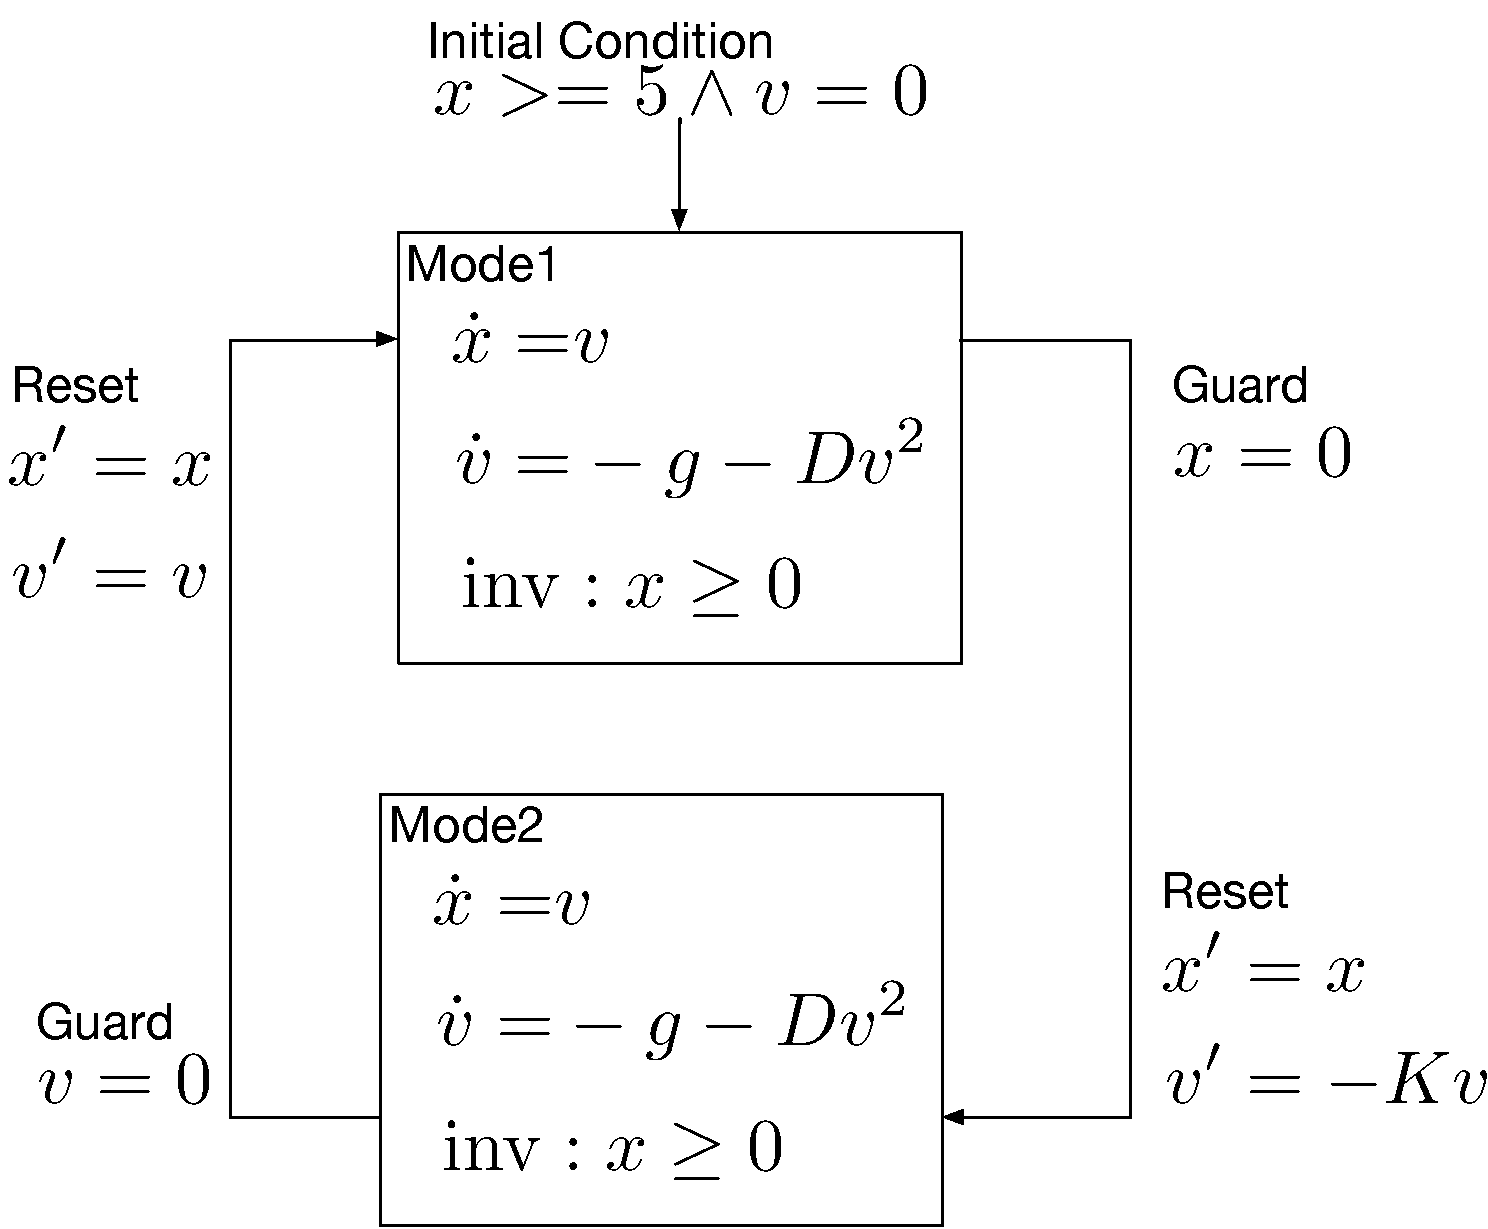
\includegraphics[width=0.5 \textwidth]{images/bouncing_ball.pdf}
  \caption{Bouncing ball example}
  \label{fig:bouncing-ball}
\end{wrapfigure}


\begin{figure}
  \centering
  \begin{Verbatim}[fontfamily=courier, frame=single, framesep=1mm,
  numbers=left, fontsize=\scriptsize]
#define D 0.45
#define K 0.9
[0, 15] x;
[9.8] g;
[-18, 18] v;
[0, 3] time;
{
  mode 1;
  invt:
        (v <= 0);
        (x >= 0);
  flow:
        d/dt[x] = v;
        d/dt[v] = -g + (- D * v ^ 1);
  jump:
        (x = 0) ==> @2 (and (x' = x) (v' = - K * v));
}
{
  mode 2;
  invt:
        (v >= 0);
        (x >= 0);
  flow:
        d/dt[x] = v;
        d/dt[v] = -g + (- D * v ^ 1);
  jump:
        (v = 0) ==> @1 (and (x' = x) (v' = v));
}
init:
@1    (and (x >= 5) (v = 0));

goal:
@1    (and (x >= 0.45));
\end{Verbatim}
  \caption{Bouncing ball example}
  \label{fig:bouncing-ball}
\end{figure}

\begin{figure}
  \centering
  \begin{Verbatim}[fontfamily=courier, frame=single, framesep=1mm,
  numbers=left, fontsize=\scriptsize]
(set-logic QF_NRA_ODE)
(declare-fun x () Real)
(declare-fun v () Real)
(declare-fun x_0_0 () Real)
(declare-fun x_0_t () Real)
...
(declare-fun x_10_0 () Real)
(declare-fun x_10_t () Real)
(declare-fun v_0_0 () Real)
(declare-fun v_0_t () Real)
...
(declare-fun v_10_0 () Real)
(declare-fun v_10_t () Real)
(declare-fun time_0 () Real)
...
(declare-fun time_10 () Real)
(declare-fun mode_0 () Real)
...
(declare-fun mode_10 () Real)
(define-ode flow_1 ((= d/dt[x] v)
                    (= d/dt[v] (+ (- 0.0 9.8) (* -0.45 (^ v 1.0))))))
(define-ode flow_2 ((= d/dt[x] v)
                    (= d/dt[v] (+ (- 0.0 9.8) (* -0.45 (^ v 1.0))))))
(assert (<= 0.0 x_0_0))
(assert (<= x_0_0 15.0))
...
(assert (<= -18.0 v_10_t))
(assert (<= v_10_t 18.0))
(assert (<= 0.0 time_0))
(assert (<= time_0 3.0))
...
(assert (<= 0.0 time_10))
(assert (<= time_10 3.0))
...

(assert (and (and (= v_0_0 0.0) (>= x_0_0 5.0)) (= mode_0 1.0) (= [x_0_t v_0_t] (integral 0. time_0 [x_0_0 v_0_0] flow_1)) (= mode_0 1.0) (forall_t 1.0 [0.0 time_0] (<= v_0_t 0.0)) (<= v_0_t 0.0) (<= v_0_0 0.0) (forall_t 1.0 [0.0 time_0] (>= x_0_t 0.0)) (>= x_0_t 0.0) (>= x_0_0 0.0) (= mode_1 2.0) (= x_0_t 0.0) (= v_1_0 (* -0.9 v_0_t)) (= x_1_0 x_0_t) (= [x_1_t v_1_t] (integral 0. time_1 [x_1_0 v_1_0] flow_2)) (= mode_1 2.0) (forall_t 2.0 [0.0 time_1] (>= v_1_t 0.0)) (>= v_1_t 0.0) (>= v_1_0 0.0) (forall_t 2.0 [0.0 time_1] (>= x_1_t 0.0)) (>= x_1_t 0.0) (>= x_1_0 0.0) (= mode_2 1.0) (= v_1_t 0.0) (= v_2_0 v_1_t) (= x_2_0 x_1_t) (= [x_2_t v_2_t] (integral 0. time_2 [x_2_0 v_2_0] flow_1)) (= mode_2 1.0) (forall_t 1.0 [0.0 time_2] (<= v_2_t 0.0)) (<= v_2_t 0.0) (<= v_2_0 0.0) (forall_t 1.0 [0.0 time_2] (>= x_2_t 0.0)) (>= x_2_t 0.0) (>= x_2_0 0.0) (= mode_3 2.0) (= x_2_t 0.0) (= v_3_0 (* -0.9 v_2_t)) (= x_3_0 x_2_t) (= [x_3_t v_3_t] (integral 0. time_3 [x_3_0 v_3_0] flow_2)) (= mode_3 2.0) (forall_t 2.0 [0.0 time_3] (>= v_3_t 0.0)) (>= v_3_t 0.0) (>= v_3_0 0.0) (forall_t 2.0 [0.0 time_3] (>= x_3_t 0.0)) (>= x_3_t 0.0) (>= x_3_0 0.0) (= mode_4 1.0) (= v_3_t 0.0) (= v_4_0 v_3_t) (= x_4_0 x_3_t) (= [x_4_t v_4_t] (integral 0. time_4 [x_4_0 v_4_0] flow_1)) (= mode_4 1.0) (forall_t 1.0 [0.0 time_4] (<= v_4_t 0.0)) (<= v_4_t 0.0) (<= v_4_0 0.0) (forall_t 1.0 [0.0 time_4] (>= x_4_t 0.0)) (>= x_4_t 0.0) (>= x_4_0 0.0) (= mode_5 2.0) (= x_4_t 0.0) (= v_5_0 (* -0.9 v_4_t)) (= x_5_0 x_4_t) (= [x_5_t v_5_t] (integral 0. time_5 [x_5_0 v_5_0] flow_2)) (= mode_5 2.0) (forall_t 2.0 [0.0 time_5] (>= v_5_t 0.0)) (>= v_5_t 0.0) (>= v_5_0 0.0) (forall_t 2.0 [0.0 time_5] (>= x_5_t 0.0)) (>= x_5_t 0.0) (>= x_5_0 0.0) (= mode_6 1.0) (= v_5_t 0.0) (= v_6_0 v_5_t) (= x_6_0 x_5_t) (= [x_6_t v_6_t] (integral 0. time_6 [x_6_0 v_6_0] flow_1)) (= mode_6 1.0) (forall_t 1.0 [0.0 time_6] (<= v_6_t 0.0)) (<= v_6_t 0.0) (<= v_6_0 0.0) (forall_t 1.0 [0.0 time_6] (>= x_6_t 0.0)) (>= x_6_t 0.0) (>= x_6_0 0.0) (= mode_7 2.0) (= x_6_t 0.0) (= v_7_0 (* -0.9 v_6_t)) (= x_7_0 x_6_t) (= [x_7_t v_7_t] (integral 0. time_7 [x_7_0 v_7_0] flow_2)) (= mode_7 2.0) (forall_t 2.0 [0.0 time_7] (>= v_7_t 0.0)) (>= v_7_t 0.0) (>= v_7_0 0.0) (forall_t 2.0 [0.0 time_7] (>= x_7_t 0.0)) (>= x_7_t 0.0) (>= x_7_0 0.0) (= mode_8 1.0) (= v_7_t 0.0) (= v_8_0 v_7_t) (= x_8_0 x_7_t) (= [x_8_t v_8_t] (integral 0. time_8 [x_8_0 v_8_0] flow_1)) (= mode_8 1.0) (forall_t 1.0 [0.0 time_8] (<= v_8_t 0.0)) (<= v_8_t 0.0) (<= v_8_0 0.0) (forall_t 1.0 [0.0 time_8] (>= x_8_t 0.0)) (>= x_8_t 0.0) (>= x_8_0 0.0) (= mode_9 2.0) (= x_8_t 0.0) (= v_9_0 (* -0.9 v_8_t)) (= x_9_0 x_8_t) (= [x_9_t v_9_t] (integral 0. time_9 [x_9_0 v_9_0] flow_2)) (= mode_9 2.0) (forall_t 2.0 [0.0 time_9] (>= v_9_t 0.0)) (>= v_9_t 0.0) (>= v_9_0 0.0) (forall_t 2.0 [0.0 time_9] (>= x_9_t 0.0)) (>= x_9_t 0.0) (>= x_9_0 0.0) (= mode_10 1.0) (= v_9_t 0.0) (= v_10_0 v_9_t) (= x_10_0 x_9_t) (= [x_10_t v_10_t] (integral 0. time_10 [x_10_0 v_10_0] flow_1)) (= mode_10 1.0) (forall_t 1.0 [0.0 time_10] (<= v_10_t 0.0)) (<= v_10_t 0.0) (<= v_10_0 0.0) (forall_t 1.0 [0.0 time_10] (>= x_10_t 0.0)) (>= x_10_t 0.0) (>= x_10_0 0.0) (= mode_10 1.0) (>= x_10_t 0.45)))
(check-sat)
(exit)
\end{Verbatim}
  \caption{Bouncing ball example}
  \label{fig:bouncing-ball}
\end{figure}

%%% Local Variables:
%%% mode: latex
%%% TeX-master: "main"
%%% End:

\section{Logical Encoding of Reachability}


The details of our encoding scheme is given in~\cite{DBLP:journals/corr/GaoKCC14}.
Here we focus on explaining how differential equations and the universal quantifications
generated by mode invariance conditions are encoded, as an extension of the SMT-LIB
~\cite{BarST-SMT-10} standard. Although such formulas are automatically generated by \dReach{}
from the hybrid system descrpition, the explanation below can be helpful for
understanding the inner mechanism of our solver.

\paragraph{Encoding integrations.}
In each mode of a hybrid system, we need to specify continuous flows defined
by systems of ordinary differential equations. We extend SMT-LIB with a command
\texttt{define-ode} to define such systems. For instance, we use $\texttt{define-ode}$ as follows to
assign a name $\mathrm{flow_1}$ to a group of ODE,
$\frac{\mathrm{d}x}{\mathrm{d}t} = v$ and
$\frac{\mathrm{d}v}{\mathrm{d}t} = -x^2$.
\begin{Verbatim}[fontfamily=courier, fontsize=\small]
(define-ode flow ((= d/dt[x] v) (= d/dt[v] -x^2)))
\end{Verbatim}
We then allow integration terms in the formula. We view the solution of system of differential equations
as a constraint between the initial-state variables, time duration, and the end-state variables. We can then write
\begin{Verbatim}[fontfamily=courier, fontsize=\small]
(integral 0 t [x_0_0 ... x_n_0] flow_i).
\end{Verbatim}
to represent
$\vec x = \vec x_0 + \int_0^t flow_i(\vec x(s))\mathrm{d}s$. Note that we do not need to explicitly mention $\vec x(s)$ as a function in the encoding, which can be inferred by the solver.

\paragraph{Universal quantification for mode invariant constriants.} To encode mode invariants in hybrid systems, we
need $\exists\forall^t$-formulas~\cite{DBLP:conf/fmcad/GaoKC13} which
is a restricted form of $\exists\forall$ formula where the universal
quantifications are limited to the time variables. In \drh{}, we
introduce a new keyword $\texttt{forall\_t}$ to encode
$\exists\forall^t$ formulas. Given a time bound $[0, time_i]$, mode
invariant f at mode $n$ is encoded into \texttt{(forall\_t n [0
  time\_i] f)}.

%%% Local Variables:
%%% mode: latex
%%% TeX-master: "main"
%%% End:

\section{Using \dReach{}}\label{sec:using-dreach}
% We now describe the input format and command line options of
% \dReach{}.
\subsection{Input Format}\label{sec:input-format}
The input format for describing hybrid systems and reachability properties consists of five
sections: macro definitions, variable declarations, mode definitions,
and initial condition, and goals. We focus on intuitive explanations here, and the formal grammar is
given in the Appendix. Figure~\ref{fig:bouncing-ball-drh} shows how to describe a small
example hybrid system, an inelastic bouncing ball with air resistance.

\begin{itemize}
\item In macro definitions, we allows users to define macros in C
preprocessor style which can be used in the following
sections. Macro expansions occur before the other parts are processed.

\item A variable declaration specifies a real variable and its domain
  in a real interval. \dReach{} requires special declaration for
  \textit{time} variable, to specify the upperbound of time duration.

\item A mode definition consists of mode id, mode invariant, flow, and jump.
\textit{id} is a unique positive interger assigned to a mode. An
invariant is a conjuction of logic formulae which must always hold in
a mode. A flow describes the continuous dynamics of a mode by providing
a set of ODEs. The first
formula of \textit{jump} is interpreted as a guard, a logic formula
specifying a condition to make a transition. Note that this allows a
transition but does not force it. The second argument of
\textit{jump}, $n$ denotes the target mode-id. The last one is
\textit{reset}, a logic formula connecting the old and new values for
the transition.

\item \textit{initial-condition} specifies the initial mode of a hybrid
system and its initial configuration. \textit{goal} shares the same
syntactic structure of \textit{initial-condition}.
\end{itemize}
\begin{figure}
  \centering
  \begin{Verbatim}[fontfamily=courier, frame=single, framesep=1mm,
  numbers=left, fontsize=\scriptsize]
#define D 0.45
#define K 0.9
[0, 15] x; [9.8] g; [-18, 18] v; [0, 3] time;
{   mode 1;
    invt: (v <= 0);  (x >= 0);
    flow: d/dt[x] = v; d/dt[v] = -g - (D * v ^ 2);
    jump: (x = 0) ==> @2 (and (x' = x) (v' = - K * v)); }
{   mode 2;
    invt: (v >= 0); (x >= 0);
    flow: d/dt[x] = v; d/dt[v] = -g + (D * v ^ 2);
    jump: (v = 0) ==> @1 (and (x' = x) (v' = v)); }
init: @1 (and (x >= 5) (v = 0));
goal: @1 (and (x >= 0.45));
\end{Verbatim}
\caption{An example of \drh{} format: Inelastic bouncing ball with air
  resistance. Lines 1 and 2 define a drag coefficient $D = 0.45$ and
  an elastic coefficient $K = 0.9$. At line 3, we declare variables
  $x, g, v,$ and $time$. At lines 4 - 7 and 8 - 11, we define two
  modes -- the falling and the bouncing-back modes respectively. At
  line 12, we specify this hybrid system to start at mode 1
  (\texttt{@1}) with initial condition satisfying
  $x \ge 5 \land v = 0$. At line 13, it asks whether we can have
  a trajectory ending at mode 1 (\texttt{@1}) while the height of the
  ball is higher than $0.45$.}
\label{fig:bouncing-ball-drh}
\end{figure}
\vspace{-1.0em}
\subsection{Command Line Options}
\dReach{} follows the standard unix command-line usage:
\begin{Verbatim}[fontfamily=courier, framesep=1mm, fontsize=\small]
dReach <options> <drh file>
\end{Verbatim}
It has the following options:
\begin{itemize}
\item If \texttt{-k <N>} is used, set the unrolling bound $k$ as $N$
  (Default: 3). It also provides \texttt{-u <N>} and \texttt{-l <N>}
  options to specify upper- and lower-bounds of unrolling bound.
\item If \texttt{--precision <p>} is used, use precision $p$ (Default: $0.001$).
\item If \texttt{--visualize} is set, \dReach{} generates extra visualization data.
\end{itemize}
We have a web-based visualization toolkit\footnote{The detailed
  instructions are available at
  \url{https://github.com/dreal/dreal/blob/master/doc/ode-visualization.md}.}
which processes the generated visualization data and shows the
counterexample trajectory. It provides a way to navigate and
zoom-in/out trajectories which helps understand and debug the target
hybrid system better.

%%% Local Variables:
%%% mode: latex
%%% TeX-master: "main"
%%% End:

\section{Example: Inelastic Bouncing Ball with Drag}
\begin{wrapfigure}{l}{0.5\textwidth}
  \centering
  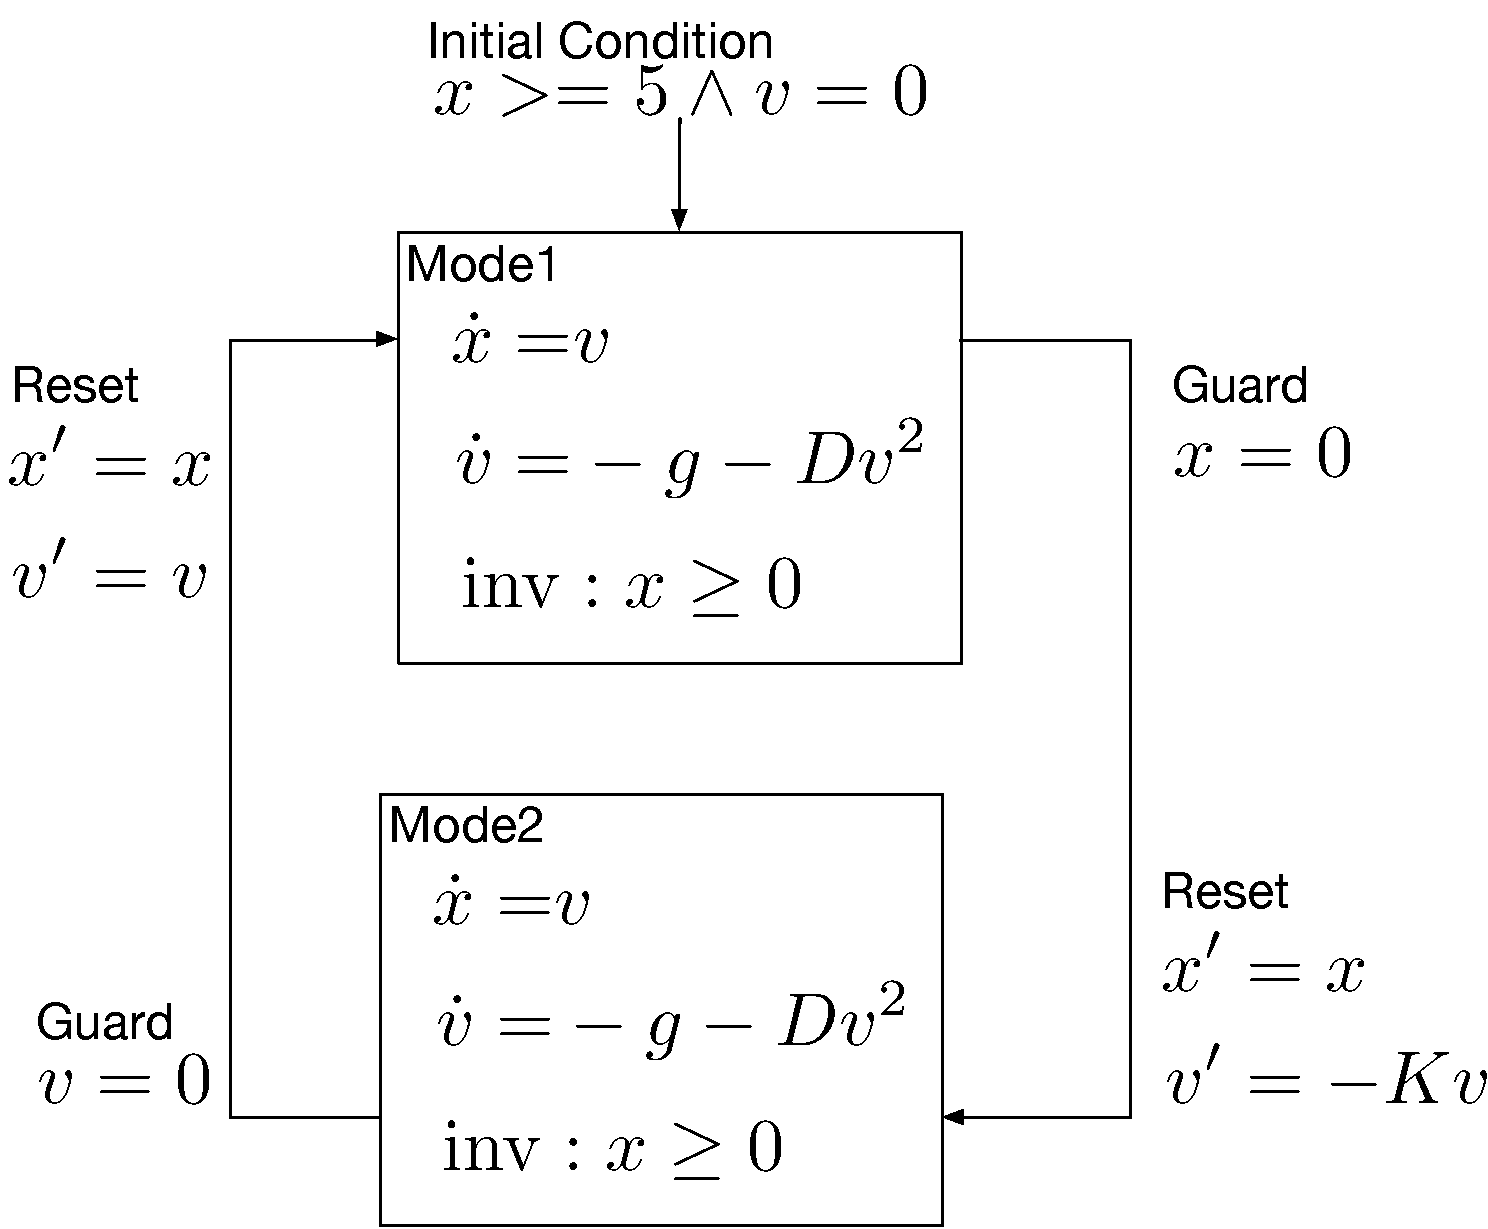
\includegraphics[width=0.5 \textwidth]{images/bouncing_ball.pdf}
  \caption{Bouncing ball example}
  \label{fig:bouncing-ball}
\end{wrapfigure}


\begin{figure}[!h]
  \centering
  \begin{Verbatim}[fontfamily=courier, frame=single, framesep=1mm,
  numbers=left, fontsize=\scriptsize]
#define D 0.45
#define K 0.9
[0, 15] x;
[9.8] g;
[-18, 18] v;
[0, 3] time;
{
  mode 1;
  invt:
        (v <= 0);
        (x >= 0);
  flow:
        d/dt[x] = v;
        d/dt[v] = -g + (- D * v ^ 1);
  jump:
        (x = 0) ==> @2 (and (x' = x) (v' = - K * v));
}
{
  mode 2;
  invt:
        (v >= 0);
        (x >= 0);
  flow:
        d/dt[x] = v;
        d/dt[v] = -g + (- D * v ^ 1);
  jump:
        (v = 0) ==> @1 (and (x' = x) (v' = v));
}
init:
@1    (and (x >= 5) (v = 0));

goal:
@1    (and (x >= 0.45));
\end{Verbatim}
  \caption{drh format of bouncing ball example}
  \label{fig:bouncing-ball-drh}
\end{figure}

\begin{figure}[!h]
  \centering
  \begin{Verbatim}[fontfamily=courier, frame=single, framesep=1mm,
  numbers=left, fontsize=\scriptsize]
(set-logic QF_NRA_ODE)
(declare-fun x () Real)
(declare-fun v () Real)
(declare-fun x_0_0 () Real)
(declare-fun x_0_t () Real)
...
(declare-fun x_10_0 () Real)
(declare-fun x_10_t () Real)
(declare-fun v_0_0 () Real)
(declare-fun v_0_t () Real)
...
(declare-fun v_10_0 () Real)
(declare-fun v_10_t () Real)
(declare-fun time_0 () Real)
...
(declare-fun time_10 () Real)
(declare-fun mode_0 () Real)
...
(declare-fun mode_10 () Real)
(define-ode flow_1 ((= d/dt[x] v)
                    (= d/dt[v] (+ (- 0.0 9.8) (* -0.45 (^ v 1.0))))))
(define-ode flow_2 ((= d/dt[x] v)
                    (= d/dt[v] (+ (- 0.0 9.8) (* -0.45 (^ v 1.0))))))
(assert (<= 0.0 x_0_0))
(assert (<= x_0_0 15.0))
...
(assert (<= -18.0 v_10_t))
(assert (<= v_10_t 18.0))
(assert (<= 0.0 time_0))
(assert (<= time_0 3.0))
...
(assert (<= 0.0 time_10))
(assert (<= time_10 3.0))
...

(assert (and (and (= v_0_0 0.0) (>= x_0_0 5.0)) (= mode_0 1.0) (=
[x_0_t v_0_t] (integral 0. time_0 [x_0_0 v_0_0] flow_1)) (= mode_0
1.0) (forall_t 1.0 [0.0 time_0] (<= v_0_t 0.0)) (<= v_0_t 0.0) (<=
...
x_9_t) (= [x_10_t v_10_t] (integral 0. time_10 [x_10_0 v_10_0]
flow_1)) (= mode_10 1.0) (forall_t 1.0 [0.0 time_10] (<= v_10_t 0.0))
(<= v_10_t 0.0) (<= v_10_0 0.0) (forall_t 1.0 [0.0 time_10] (>= x_10_t
0.0)) (>= x_10_t 0.0) (>= x_10_0 0.0) (= mode_10 1.0) (>= x_10_t
0.45))) (check-sat) (exit)
\end{Verbatim}
  \caption{SMT2 encoding of the bounded reachability problem of
    bouncing ball ($k = 3$) }
  \label{fig:bouncing-ball-smt2}
\end{figure}

%%% Local Variables:
%%% mode: latex
%%% TeX-master: "main"
%%% End:

\bibliographystyle{abbrv}
\bibliography{tau_tacas}

\section*{Appendix}
\section{Experiments}
\vspace{-.1cm}
Our method is implemented in the open-source tool {\bf SReach} (\url{https://github.com/rachelwang/SReach}). See Appendix \ref{apndx:usage} for its usage. All benchmarks and data shown below are on the tool website. All experiments were conducted on a machine with 2.9GHz Intel Core i7 processor and 8GB RAM, running OS X 10.9.2. 
In our experiments we used $0.001$ as the precision for the $\delta$-decision problem; and Bayesian sequential estimation
with $0.01$ half-interval width, coverage probability $0.99$, and uniform prior ($\alpha = \beta = 1$). The 
detailed description of the following models in Appendix \ref{apndx:model} demonstrates their highly nonlinear and nondeterministic characteristics.

{\bf\noindent Prostate cancer treatment.}
%\textit{Model Description}.
We modified the model of the intermittent androgen suppression (IAS) therapy in \cite{tanaka2010mathematical} by adding parametric uncertainty. The IAS therapy switches between  treatment-on, and treatment-off with respect to the serum level thresholds of prostate-specific antigen (PSA) - $r_0$ and $r_1$. As suggested by the clinical trials \cite{bruchovsky2006final}, an effective IAS therapy highly depends on the individual patient. Thus, we modified the model by taking the parametric variation caused by the personalized differences into account. In details, according to the clinic data from hundreds of patients \cite{bruchovsky2007locally}, we replaced 6 system 
parameters with random variables with appropriate (continuous) distributions, including $\alpha_x$ (proliferation rate of AD cells), $\alpha_y$ (proliferation rate of AI cells), $\beta_x$ (apoptosis rate of AD cells), $\beta_y$ (apoptosis rate of AI cells), $m_1$ (mutation rate from AD to AI cells), and $z_0$ (normal androgen level).
\vspace{-.5cm}
\begin{table}[th!]
\captionsetup{font=scriptsize}
\centering
    \begin{tabular}{c|c|c|c|c|c|c|c|c}
    \hline
    Model & \#RVs & $r_0$ & $r_1$ & Est\_P & \#S\_S & \#T\_S & Avg\_T(s) & Tot\_T(s) \\ \hline
    PCT1  & 6     & 5.0  & 10.0 & 0.04   & 0      & 227    & 0.145   & 32.915     \\ \hline
    PCT2  & 6     & 7.0  & 11.0 & 0.591  & 2144   & 3628   & 432.491 & 1569077.348     \\ \hline
    PCT3  & 6     & 10.0 & 15.0 & 0.996  & 227    & 227    & 692.861   & 157279.446   \\ \hline
    \end{tabular}
    \caption{\#RVs = number of random variables in the model, \#S\_S = number of $\delta$-sat samples, 
\#T\_S = total number of samples, $r_0$ = lower threshold of the serum PSA level, $r_1$ = upper threshold, 
Est\_P = estimated probability of the property,  Avg\_T(s) = average CPU time of each sample in seconds, and Tot\_T(s) = total CPU time for all samples in seconds.}
    \label{table:prostate}
\end{table}
\vspace{-1.1cm}
%\subsection{Cardiac models}
%\textit{Experiments and Results} 

To describe the variations due to individual difference, we assigned $\alpha_x$ to be $U(0.0193, 0.0214)$, $\alpha_y$ to be $U(0.0230, 0.0254)$, $\beta_x$ to be $U(0.0072, 0.0079)$, $\beta_y$ to be $U(0.0160, 0.0176)$, $m_1$ to be $U(0.0000475, 0.0000525) $, and $z_0$ to be $N(30.0, 0.001)$. 
We used {\bf SReach} to estimate the probabilities of the model preventing the relapse of the prostate cancer with three distinct pairs of treatment thresholds (\ie, combinations of $r_0$ and $r_1$).  In the experiments, we chose 2 as the unfolding steps. For each sample generated, {\bf SReach} dealt with $41$ variables, and $10$ ODEs. As shown in Table \ref{table:prostate}, the model with thresholds $r_0 = 10$, and $r_1 = 15$ has the probability approaching to 1, indicating that these thresholds can be considered for the general treatment. 

{\bf\noindent Atrial Fribrillation.} The minimum resistor model (MRM) reproduces experimentally measured characteristics 
of human ventricular cell dynamics \cite{bueno2008minimal}. 
The MRM reduces the complexity of existing models by representing channel gates of different ions with one fast channel, and two slow gates. However, due to this reduction, for most model parameters, it becomes impossible to obtain their values through measurements. With this application, we will show that {\bf SReach} can also be adopted to identify appropriate ranges and distributions for model parameters, \ie, parameter estimation.

%\textit{Experiments and Results} 
To illustrate the way that {\bf SReach} is used to conduct parameter estimation, we chose two system parameters - $EPI\_TO1$, and $EPI\_TO2$, and varied their distributions to see with which distributions for these two system parameters, the model can present the desired pattern. The model has 4 modes. In the experiments, we chose $3$ as the unfolding steps. For each sample generated, {\bf SReach} dealt with $62$ variables, and $24$ ODEs. As in the Table \ref{table:cardiac}, when $EPI\_TO1$ is either close to $400$, or between $0.0061$ and $0.007$, and $EPI\_TO2$ is close to $6$, the model can satisfy the given bounded reachability property with a probability very close to $1$. 
\vspace{-.5cm}
\begin{table}[h!]
\captionsetup{font=scriptsize}
\centering
    \begin{tabular}{c|c|c|c|c|c|c|c|c}
    \hline
    Model         & \#RVs & EPI\_TO1            & EPI\_TO2         & \#S\_S & \#T\_S & Est\_P &  A\_T(s) & T\_T(s) \\ \hline
    Cd\_to1\_s    & 1     & U(6.1e-3, 7e-3)    & 6              & 227       & 227      & 0.996     & 0.362   & 82.174     \\ \hline
    Cd\_to1\_uns  & 1     & U(5.5e-3, 5.9e-3)   & 6              & 0         & 227      & 0.004     & 0.124 & 28.148       \\ \hline
    Cd\_to2\_s    & 1     & 400               & U(0.131, 6)    & 227       & 227      & 0.996     & 0.361  & 81.947      \\ \hline
    Cd\_to2\_uns  & 1     & 400               & U(0.1, 0.129)    & 0         & 227      & 0.004     & 0.139   & 31.552     \\ \hline
    Cd\_to12\_s   & 2     & N(400, 1e-4)      & N(6, 1e-4)     & 227       & 227      & 0.996     & 0.373  & 84.671      \\ \hline
    Cd\_to12\_uns & 2     & N(5.5e-3, 10e-6) & N(0.11, 10e-5) & 0         & 227      & 0.004     & 0.131  & 29.737      \\ \hline
    \end{tabular}
    \caption { \#RVs = number of random variables in the model, \#S\_S = number of $\delta$-sat samples, 
\#T\_S = total number of samples, Est\_P = estimated probability of property,  A\_T(s) = average 
CPU time of each sample in seconds, and T\_T(s) = total CPU time for all samples in seconds.}
    \label{table:cardiac}
\end{table}
\vspace{-1cm}

\begin{comment}

\subsection{Application to the stabilization control of quadcopters}

\textit{Model Description}.
We modeled the stabilization control of a quadcopter, and are interested in analyzing its robustness. In other words, given an arbitrary initial location and position, this model will guarantee that the quadcopter will soon become stable via adjusting velocities of four rotors. To specify the arbitrary initial status, we introduced 6 random variables: ($x_0$, $y_0$, $z_0$) (the initial location),  $\phi_0$ (the initial roll angle), $\theta_0$ (the initial pitch angle), and $\psi_0$ (the initial yaw angle).

\textit{Experiments and Results}. To validate this model, {\bf SReach} was adopted with the BIFT statistical testing option.  

\end{comment}

{\noindent\bf Additional benchmarks.} To further demonstrate the feasibility of {\bf SReach}, we also applied it to the following benchmarks. 
Table \ref{table:exp} shows the results of experiments. BB refers to the bouncing ball models, 
Tld the thermostat model with linear temperature decrease, Ted the thermostat model with exponential decrease, 
DT the dual thermostat models, W the watertank models, DW the dual watertank models, 
%Gear the gear shift control model, 
Que the model for queuing system, 3dOsc the model for 3d oscillator, and QuadC the model for quadcopter 
stabilization control. 
\vspace{-.5cm}
\begin{table}[h!]
\captionsetup{font=scriptsize}
\centering
    \begin{tabular}{c|c|c|c|c|c|c|c|c|c|c|c}
    \hline
    Benchmark & \#Ms & K & \#ODEs & \#Vs & \#RVs & $\delta$ & Est\_P & \#S\_S & \#T\_S &  A\_T(s) & T\_T(s)  \\ \hline
    BBK1      & 1       & 1 & 2      & 14    & 3     & 0.001 & 0.754  & 5372      & 7126     & 0.086  & 612.836         \\ \hline
    BBK5      & 1       & 5 & 2      & 38    & 3     & 0.001 & 0.059  & 209       & 3628     & 0.253   &  917.884       \\ \hline
    BBwDv1    & 2       & 2 & 4      & 20    & 4     & 0.001 & 0.208  & 2206      & 10919    & 0.080   &  873.522     \\ \hline
    BBwDv2K2  & 2       & 2 & 4      & 20    & 3     & 0.001 & 0.845  & 7330      & 8669     & 0.209    & 1811.821      \\ \hline
    BBwDv2K8  & 2       & 8 & 4      & 56    & 3     & 0.001 & 0.207  & 2259      & 10901    & 0.858  & 9353.058        \\ \hline
    Tld       & 2       & 7 & 2      & 33     & 4     & 0.001 & 0.996      & 227         & 227        & 0.213     & 48.351         \\ \hline
    Ted       & 2       & 7 & 4      & 50     & 4     & 0.001 & 0.996      & 227         & 227       & 12.839   & 2914.448     \\ \hline
    DTldK3    & 2       & 3 & 4      & 26    & 2     & 0.001 & 0.996  & 227       & 227      & 0.382    & 86.714      \\ \hline
    DTldK5    & 2       & 5 & 4      & 38    & 2     & 0.001 & 0.161  & 1442      & 8961     & 0.280  &  2509.078       \\ \hline
    W4mv1       & 4       & 3 & 8      & 26     & 6     & 0.001 & 0.381      & 5953         & 15639        & 0.238   & 3722.082     \\ \hline
    W4mv2K3       & 4       & 3 & 8      & 26     & 6     & 0.001 & 0.996      & 227         & 227        & 0.673   & 152.771      \\ \hline
    W4mv2K7       & 4       & 7 & 8      & 50     & 6     & 0.001 & 0.004     & 0         & 227        & 0.120    & 27.240          \\ \hline
    DWK1      & 2       & 1 & 4      & 14    & 5     & 0.001 & 0.996  & 227       & 227      & 0.171   & 38.817      \\ \hline
    DWK3      & 2       & 3 & 4      & 26    & 5     & 0.001 & 0.996  & 227       & 227      & 0.215    & 48.806      \\ \hline
    DWK9      & 2       & 9 & 4      & 62    & 5     & 0.001 & 0.996  & 227       & 227      & 5.144   &  1167.688      \\ \hline
   % Gear      & 4       & ~ & ~      & ~     & ~     & 0.001 & ~      & ~         & ~        & ~     & ~          \\ \hline
    Que       & 3       & 2 & 3      & 13     & ~     & 0.001 & 0.228      & 2662         & 11677        & 0.095   & 1109.315   \\ \hline
    3dOsc     & 3       & 2 & 18      & 48     & 2     & 0.001 & 0.996      & 227         & 227        & 8.273  & 1877.969   \\ \hline
    QuadC     & 1       & 0 & 14      & 44     & 6     & 0.001 & 0.996      & 227         & 227        & 825.641 & 187420.507   \\ \hline
    \end{tabular}
    \caption {\#Ms = number of modes, K indicates the unfolding steps, \#ODEs = number of ODEs in the model, \#Vs = number of total variables in the unfolded formulae, \#RVs = number of random variables in the model, $\delta$ = precision used in 
{\bf dReach}, \#S\_S = number of $\delta$-sat samples , \#T\_S = total number of samples, Est\_P = estimated 
probability of the property,  A\_T(s) = average CPU time of each sample in seconds, and T\_T(s) = total CPU time for all samples in seconds.}
    \label{table:exp}
\end{table}
\vspace{-1.1cm}


\end{document}
